\section{Simulation}
Le but est de générer une matrice d'adjacence A sous les mêmes hypothèses que \eqref{eq:1} en faisant varier les différents paramètres, à savoir: $n$, $p_{in}$, $p_{out}$ \\

\begin{figure}[h]
\centering
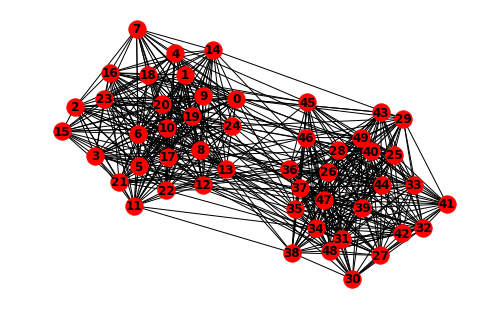
\includegraphics[scale=0.6]{static/graph_n50_pin08_pout01.png}
\caption{Graphe généré à partir des paramètres: $n=50$, $p_{in}=0.8$, $p_{out}=0.1$}
\end{figure}

L'élément discriminant du test spectral étant la variable $ \Delta p= p_{in} - p_{out}$, nous allons tester 3 valeurs représentatives des différents types de résultats:
\begin{itemize}
	\item[1-] $\Delta p \in [-1,\: 0] \implies$ le graphe ne comporte pas de structure de communauté ;
	\item[2-] $\Delta p \in [0,\: p_{lim}] \implies$ le graphe comporte une structure de communauté mais la méthode spectrale ne réussi pas à la trouver ;
	\item[2-] $\Delta p \in [p_{lim},\: 1] \implies$ le graphe comporte une structure de communauté.\\
\end{itemize}

Par la suite nous allons tester pour les valeurs $\Delta p= 0.5, 0.08, -0.5$ .
De plus nous ferons une première vague de test avec $n=100$ et une autre avec $n=1000$.
La terminologie utilisée dans les figures ci-dessous est:
\begin{itemize}
	\item[- \underline{$n,\: p_{in},\: p_{out},\: p_{lim},\: z1,\: z2$}:] sont identiques aux notations utilisées jusqu'à présent ;
	\item[- \underline{$z1\: theoric, \:z2\: theoric$}:] sont les plus grandes valeurs propres $z1$ et $z2$ calculées via les équations \eqref{z1} et \eqref{z2} ;    
	\item[- \underline{$p_{in}\: estimated, \:p_{out}\: estimated$}:] sont les probabilités du SBM calculées a posteriori grâce aux valeurs propres $z1$ et $z2$.\\
\end{itemize}
Les $p_{in}\: estimated, \:p_{out}\: estimated$ sont calculés via un calcul d'optimisation (la fonction ``fsolve'' en python).
\begin{figure}[H]
	\begin{subfigure}{.5\textwidth}
		\centering
		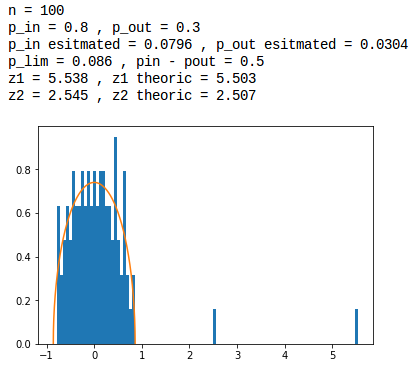
\includegraphics[scale=0.58]{static/spectral_n100_pin08_pout03.png}
		\caption{$n=100$, $\Delta p=0.5$}
	\end{subfigure}
	\begin{subfigure}{.5\textwidth}
		\centering
		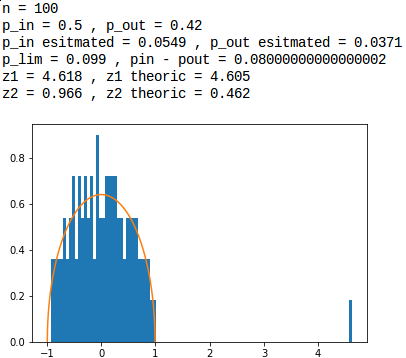
\includegraphics[scale=0.58]{static/spectral_n100_pin05_pout042.png}
		\caption{$n=100$, $\Delta p=0.08$}
	\end{subfigure}
	\begin{subfigure}{.5\textwidth}
		\centering
		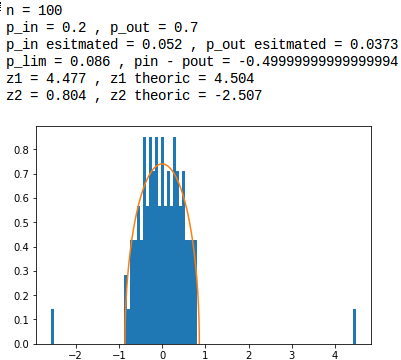
\includegraphics[scale=0.58]{static/spectral_n100_pin02_pout07.png}
		\caption{$n=100$, $\Delta p=-0.5$}
	\end{subfigure}
	\begin{subfigure}{.5\textwidth}
		\centering
		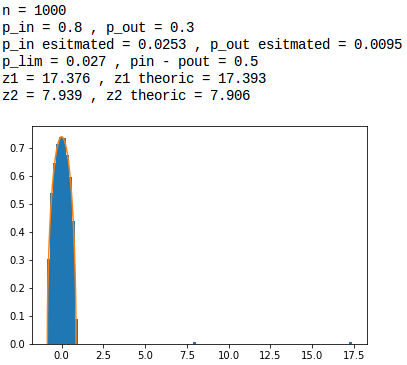
\includegraphics[scale=0.58]{static/spectral_n1000_pin08_pout03.png}
		\caption{$n=1000$, $\Delta p=0.5$}
	\end{subfigure}
	\begin{subfigure}{.5\textwidth}
		\centering
		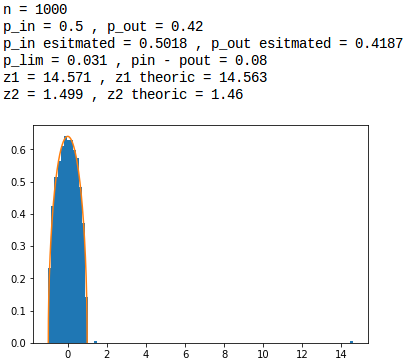
\includegraphics[scale=0.58]{static/spectral_n1000_pin05_pout042.png}
		\caption{$n=1000$, $\Delta p=0.08$}
	\end{subfigure}
	\begin{subfigure}{.5\textwidth}
		\centering
		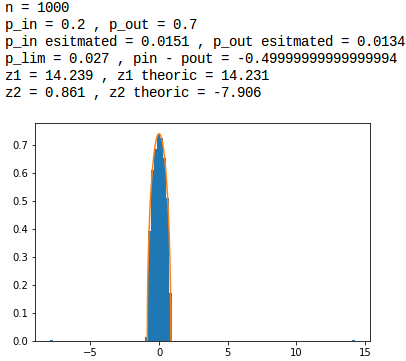
\includegraphics[scale=0.58]{static/spectral_n1000_pin02_pout07.png}
		\caption{$n=1000$, $\Delta p=-0.5$}
	\end{subfigure}
\end{figure}

La première observation que l'on peut faire est que les valeurs propres de nos matrices d'adjacence sont bien distribuées selon la loi du demi-cercle de Wigner.
De plus, en fonction de $\Delta p$ la mesure spectrale est perturbé (ou pas) par une ou deux valeurs propres qui sortent du support de la distribution initiale.\\

Dans les cas avec $\Delta p = 0.5$ on voit très clairement deux valeurs propres qui se détachent du support de la distribution de Wigner.
Les valeurs $z1$, $z2$ correspondent bien aux valeurs théoriques et dans ce cas on retrouve, avec un taux d'erreur de l'ordre de $10^{-2}$, les valeurs $p_{in}$, $p_{out}$ du modèle utilisé pour générer le graphe.\\
Dans les cas avec $\Delta p = -0.5$ on ne s'attend pas à ce que les valeurs théorique du modèles correspondent aux valeurs trouvées par la simulation dans la mesure où il n'y a en théorie aucune structure de communauté dans le graphe.
Cependant, on observe valeur propre en dehors du support de la loi de Wigner négative.
Par conséquent lorsque l'on obtient une valeur propre négative, le modèle spectral définit ci-dessus nous permet de conclure qu'il n'y a pas de structure de communauté dans le graphe.\\
Enfin, dans le cas avec $\Delta p = 0.08$, il y a en théorie une structure de communauté. 
Cependant on se retrouve dans le cas limite décrit dans \autoref{subsec:1.3}  
